\subsection{Prime-Time Ratio} \label{subsec:primetime}

ISP providers need to design networks capable of handling the heaviest total usage
in a day. Such heavy demand is usually observed during prime time hours in the 
evening, when many subscribers heavily consume real-time entertainment traffic
(video) (seen as primarily responsible for high usage during these hours).
The FCC defines prime-time as the local time from 7:00 PM to 11:00 PM.
\cite{fcc2014measuring-broadband}. To measure the concentration of network usage
during prime-time, we use Sandvine's definition of the \emph{Prime-Time 
ratio}: the ratio of the average (hourly) traffic demand during prime-time hours to the average 
demand in non-prime-time hours.\cite{sandvine20141h, sandvine20142h}.

We measure the prime-time ratio of the subscribers in the control and treatment groups
considering each contiguous four hour periods of a day. In our datasets we find the
evening hours with the largest prime-time ratio are 8:00 PM -- 12:00 AM.

%\begin{figure}[t]
%\begin{minipage}{1\linewidth}
%\centering
%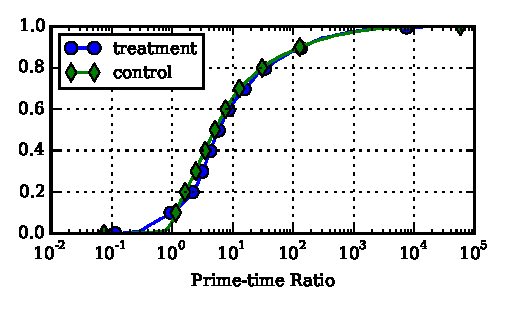
\includegraphics[width=1\linewidth]{figures/prime-time-ratio-per-device-cdf-MEAN.pdf}
%\caption{Prime-Time Ratio\label{fig:cdf-prime-time-ratio}}
%\end{minipage}
%\end{figure}

%\begin{subfigure}[]{.32\linewidth}
%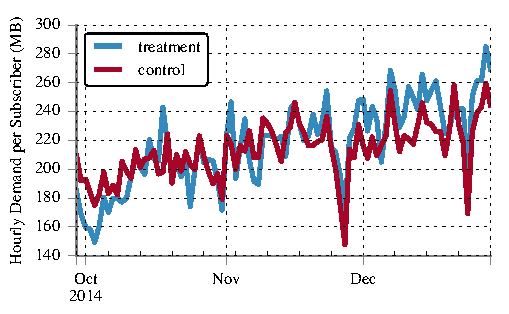
\includegraphics[width=1\linewidth]{figures/primetime_usage_per_day_per_subs.pdf}
%\caption{\label{fig:pt}}
%\end{subfigure}

%\begin{subfigure}[b]{.32\linewidth}
%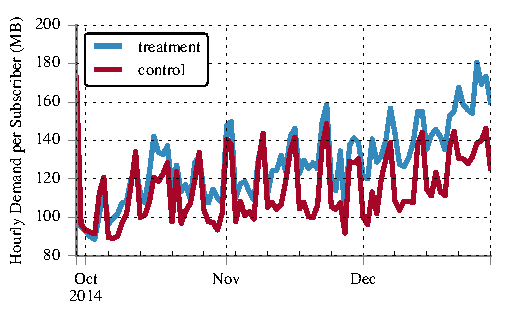
\includegraphics[width=1\linewidth]{figures/nonprimetime_usage_per_day_per_subs.pdf}
%\caption{\label{fig:non-pt}}
%\end{subfigure}


Table~\ref{tab:data-stats} shows that the hourly downlink traffic per 1000 subscribers between 8:00 PM -- 12:00 AM is 
209.5 GB for \treatment{}, and 205.1 GB for \control{}. However, during an average hour
outside of prime time, the traffic per 1000 subscribers is 122.3 GB for the higher tier
and 108.5 GB for the lower tier. This difference in demand during hours outside of the
daily prime-time is also apparant from the weekly usage patterns in Figure~\ref{fig:traffic-demand-timeseries}.

\begin{table}[t]
\begin{tabular}{| cc | c |c | }\hline
  &                    & Weekday         & Weekends \\\hline
\multirow{2}{*}{\begin{tabular}[c]{@{}l@{}}Hourly Traffic in\\ Prime-Time\end{tabular}}
& treatment          & 233.12          & 246.93   \\
& control            & 225.40          & 238.15   \\\hline
\multirow{2}{*}{\begin{tabular}[c]{@{}l@{}}Hourly Traffic in\\ Non-Prime-Time\end{tabular}}
& treatment & 124.18 & 143.08    \\
& control   & 104.30  & 133.16  \\\hline
\multirow{2}{*}{\begin{tabular}[c]{@{}l@{}}Prime-Time Ratio\end{tabular}}
& treatment & \textbf{1.88} &  1.73 \\
& control  &  \textbf{2.16} &  1.79 \\\hline
\end{tabular}
\caption{Hourly Traffic Demand during in prime-time hours (MB)\label{prime-time-demand}}
\end{table}


We calculate the prime-time ratio per day over weekends and weekdays,
as shown in Table \ref{prime-time-demand}.
%in figure~\ref{fig:cdf-prime-time-ratio}. A comparison shows 
On weekends, the prime-time ratios for both groups are
1.73 and 1.79 respectively. On the weekdays, the prime-time ratio for \control{}
is much higher, 2.16, as compared to \treatment{}, 1.88. The demand
during prime-time hours on the weekdays on the higher tier is within 4\% of
the traffic on the lower tier. In contrast, the demand in non-prime-time hours
(outside 8:00 PM -- 12:00 PM) is much higher for the treatment group, especially on weekdays. 

For our dataset, the prime-time ratio for the treatment and control groups
were 1.70 and 1.93 respectively. By definitition, the prime-time ratio is measured using
total traffic volume in a day. However, not all subscribers contribute equally
to the traffic volume. We observed that the median \emph{prime-time ratio per subscriber}
is 3.39 for the \treatment{} group and 2.91 for the \control{} group. 
The prime time ratio of the higher tier is more than the lower tier when calculated per
subscriber, but by volume it is the inverse.
The overall demand of subscribers in the \treatment{} may have decreased by 
total volume of traffic, however, it has increased on a per-subscriber basis.
This result indicates that individual subscribers that do not contribute substantially
to the traffic volume are the ones who have higher usage in prime-time as compared to their
lower tier counterparts.

We observerd 9\% of the \control{} group and 14\% of 
the treatment group had prime-time ratios less than 1. Such subscribers 
have a larger aggregate demand during non-prime-time hours. These
may be small home-run businesses, users who work at home, or 
users who have unexpected usage behaviors. We also found 6\% of the 
subscribers in both groups had a prime-time ratio over 100.
